\section{Teil}
beinhaltet folgende Foliensätze:

\begin{itemize}
    \item Teil 3a:  Produktarchitektur, Modularisierung
    \item Teil 3b:  Design Structure Matrix

\end{itemize}

% subsection
%-------------------------------------------------------------------------------------------
\subsection{Welche drei Schritte sind zur Bildung einer Modularen Produktarchitektur relevant?}

\begin{itemize}
    \item \textbf{Identifikation der Komponenten}
        \begin{itemize}
            \item Produkt in Komponenten zerlegt, um Module zu bilden.
            \item Granularität beschreibt den Grad der Zerlegung.
            \item Granularität muss zu Komplexität und Zielen passen.
        \end{itemize}
    \item \textbf{Analyses der Abhängigkeiten von Komponenten}
        \begin{itemize}
            \item Interaktionen oder Abhängigkeiten der Komponenten untereinander analysieren.
            \item z.B.: Mechanische Schnittstellen mit modularer Bauweise - mechanische Interaktion der Komponenten analysieren.
        \end{itemize}
    \item \textbf{Gruppierung zu Modulen}
        \begin{itemize}
            \item Komponenten zu Module zusammenfassen.
        \end{itemize}
\end{itemize}

% subsection
%-------------------------------------------------------------------------------------------
\subsection{Welche Funktions- und Bausteinarten in Baukästen kennen Sie?}

\begin{itemize}
    \item \textbf{Grundfunktionen}
        \begin{itemize}
            \item Grundlegende, immer wiederkehrende Funktionen.
            \item Mit anderen Grundfunktionen zur Bildung der Gesamtfunktion.
        \end{itemize}
    \item \textbf{Hilfsfunktionen}
        \begin{itemize}
            \item Funktion Verbinden und Anschließen.
            \item Kopplung zwischen Funktionsbausteinen. 
        \end{itemize}
    \item \textbf{Sonderfunktionen}
        \begin{itemize}
            \item Spezielle, ergänzende oder spezifische Teilfunktionen zu Bildung der Gesamtfunktion.
        \end{itemize}
    \item \textbf{Anpassungsfunktionen}
        \begin{itemize}
            \item Schnittstelle zur Umwelt mit anderen Systemen. 
            \item Auftragsspezifisch anzupassen.
            \item System wird mechanisch, elektrisch und informationstechnisch mit Umwelt verbunden.
        \end{itemize}
    \item \textbf{Auftragsspezifische Funktionen}
        \begin{itemize}
            \item Für projektspezifische Funktionen, welche nicht standardmäßig angeboten werden.
        \end{itemize}
    \item \textbf{MUSS – Funktionen}
        \begin{itemize}
            \item Umfassen Grund-, Hilfs-, und Anpassungsfunktionen. 
            \item Zwingend notwendig zur Bildung der Gesamtfunktion. 
        \end{itemize}
    \item \textbf{KANN – Funktionen}
        \begin{itemize}
            \item Aus Sonderfunktionen gebildet.
            \item Nice to Have-Elemente.
        \end{itemize}
\end{itemize}


% subsection
%-------------------------------------------------------------------------------------------
\subsection{Was sind Vor- und Nachteile von Produktplattformen?}

\textbf{Vorteile}
\begin{itemize}
    \item Einfache Erstellung von Varianten. Anpassung an geänderte Varianten.
    \item Abdeckung weiterer Marktsegmente bei geringem Aufwand.
    \item Komponenten trotzdem in großen Stückzahlen produzierbar (Kostenvorteil).
\end{itemize}

\textbf{Nachteile}
\begin{itemize}
    \item Zusätzlicher Aufwand für die Verwaltung der Varianten.
    \item Hoher Planungsaufwand zu Beginn.
\end{itemize}

% subsection
%-------------------------------------------------------------------------------------------
\subsection{Was versteht man unter Kundenindividuelle Massenproduktion?}

Kompromiss aus Massenfertigung und individueller Anpassung. Massenproduktion ist effizient, aber nicht auf Kundenwunsch anpassbar. Einsatz von Produktplattformen. 

z.B. Autoindustrie: Selbes Modell in vielen unterschiedlichen Varianten (Farbe, Ausstattung, ...).


% subsection
%-------------------------------------------------------------------------------------------
\subsection{Was ist ein Graph und welche Arten gibt es?}

\begin{itemize}
    \item Mathematische Grundlage zur Darstellung eines beliebigen Netzwerks.
    \item Ursprung: Königsberger Brückenproblem.
    \item Zur generischen Beschreibung von Netzwerken.
    
    \begin{figure}[H]
        \centering
        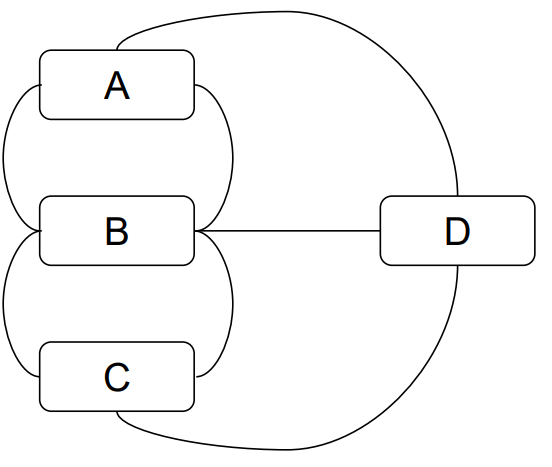
\includegraphics[width=0.6\linewidth]{Bilder/Teil3_Graph_Allgemein.png}
        \caption{Graph allgemein}
    \end{figure}

    \item \textbf{Eigenschaften:}
        \begin{itemize}
            \item Gerichtet, Ungerichtet oder beides
            \item Knoten als auch Kanten können gewichtet sein.
            \item Kante kann zu Ursprungsknoten führen.
            \item Keine, eine oder mehrere Kanten können zwei Knoten verbinden.
            \item Offene oder lose Enden.
        \end{itemize}
    \item \textbf{Charakteristiken:}
        \begin{itemize}
            \item Unterscheidung Knoten und Kanten.
            \item Zwei Kanten angrenzend, wenn sie sich einen Knoten teilen.
            \item Knoten aneinander angrenzend, wenn sie sich eine Kante teilen.
            \item Eine Kante kann zu einem Knoten führen oder weggehen.
            \item Anzahl der Kanten zu einem Knoten bestimmt dessen Ordnung.
        \end{itemize}
    \item \textbf{Arten von Graphen:}
        \begin{itemize}
            \item Ungerichtet, Gerichtet, Beides
            \begin{figure}[H]
                \centering
                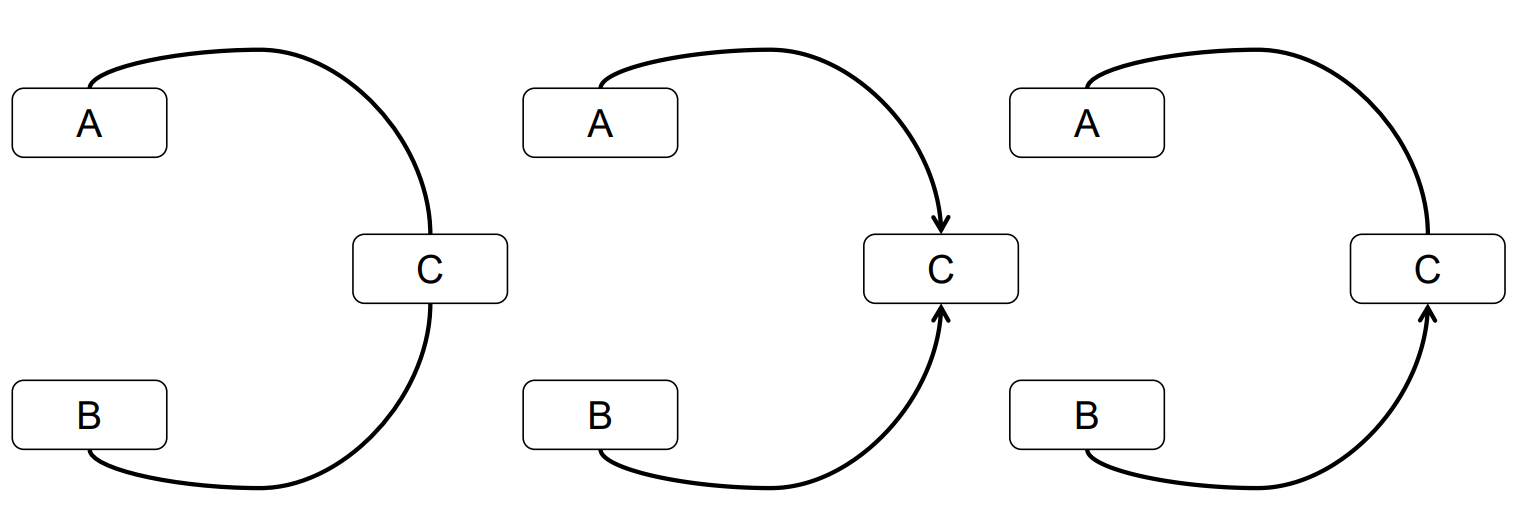
\includegraphics[width=0.7\linewidth]{Bilder/Teil3_ArtenGraphen.png}
                \caption{Arten von Graphen}
            \end{figure}
        \end{itemize}
\end{itemize}


% subsection
%-------------------------------------------------------------------------------------------
\subsection{Erklären Sie einen gewichteten Graphen?}
Ein Gewichteter Graph hat \textbf{Gewichtungsfaktoren} für die Knoten und Kanten.

z.B. Kosten, Bearbeitungs- und Transportzeit

\begin{figure}[H]
    \centering
    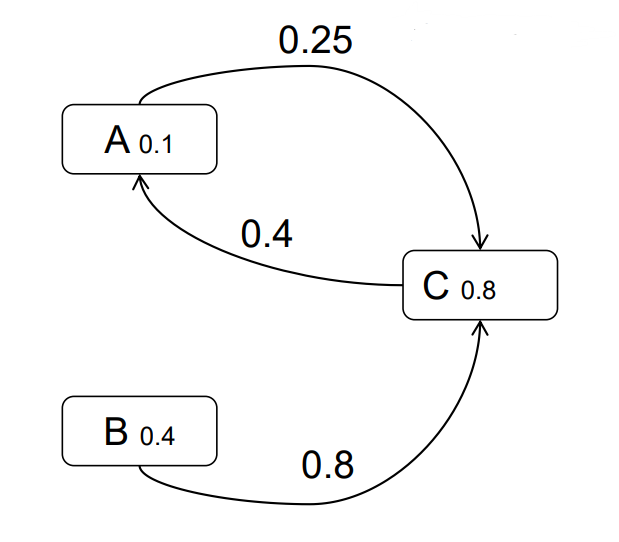
\includegraphics[width=0.6\linewidth]{Bilder/Teil3_GewichteterGraph.png}
    \caption{Beispiel Gewichteter Graph}
\end{figure}


% subsection
%-------------------------------------------------------------------------------------------
\subsection{Wofür steht der Begriff DSM?}
\textbf{Design Structure Matrix}
\begin{itemize}
    \item Zeigt Verbindungen zwischen Systemelementen in Matrixform.
    \item Elemente (z.B. Aktivitäten eines Prozesses) in Zeilen und Spalten einer symmetrischen Matrix anhand logischer Abhängigkeiten aufgetragen. 
    \item Leserichtung aufgetragen: \textbf{Zeile beeinflusst Spalte}
    \item Diagonale bleibt unbeachtet.
    \item DSM innerhalb einer Domäne modellieren, um Aussagefähigkeit zu gewähleisten.
    \item \textbf{Vorteile:}
        \begin{itemize}
            \item Einfache und präzise Möglichkeit komplizierte Systeme darzustellen.
            \item Erlaubt Einsatz von leistungsfähigen Analysemöglichkeiten (Clustering, Sequenzierung, Matrixanalysen).
        \end{itemize}
    \item \textbf{Nachteile:}
        \begin{itemize}
            \item Knoten referenzieren nicht auf Kanten.
            \item Eigenschaften der Kanten können nur bedingt dargestellt werden.
            \item Zeitliche Änderungen der Struktur schwierig darzustellen.
            \item Schwierig zu managen bei hierarchischer Aufteilung.
        \end{itemize}
\end{itemize}

\begin{figure}[H]
    \centering
    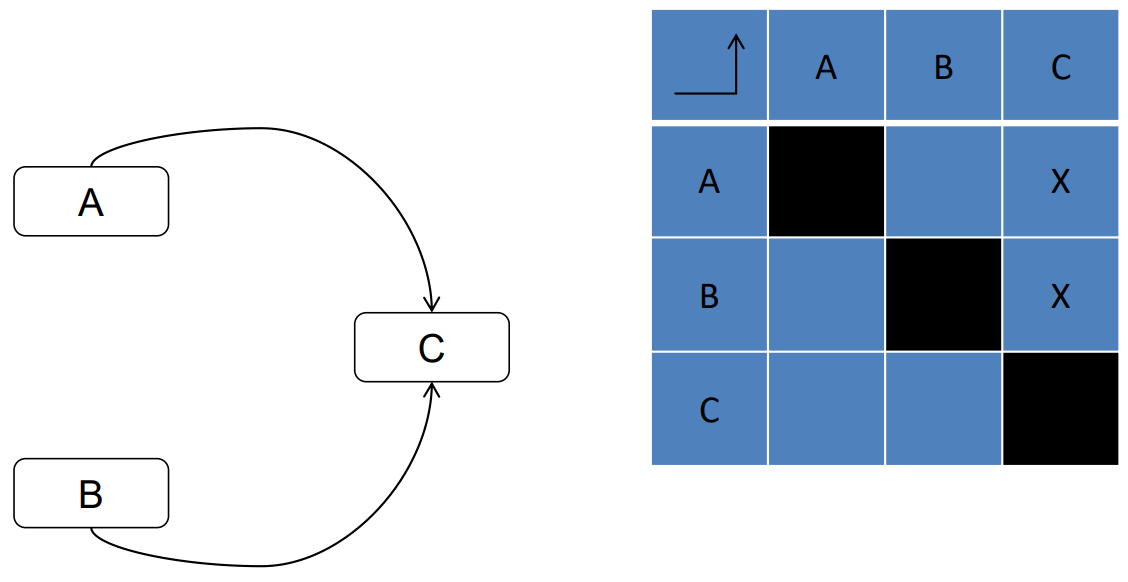
\includegraphics[width=0.6\linewidth]{Bilder/Teil3_MatrixRepresentationGerichtet.png}
    \caption{Beispiel Matrix Representation gerichteter Graph}
\end{figure}


% subsection
%-------------------------------------------------------------------------------------------
\subsection{Welche Arten von DSM gibt es?}

\begin{itemize}
    \item \textbf{Komponentenbasiert}
        \begin{itemize}
            \item Verbindungen von Komponenten.
            \item Anwendung in Systemarchitektur, Systems Engineering und System Design.
            \begin{figure}[H]
                \centering
                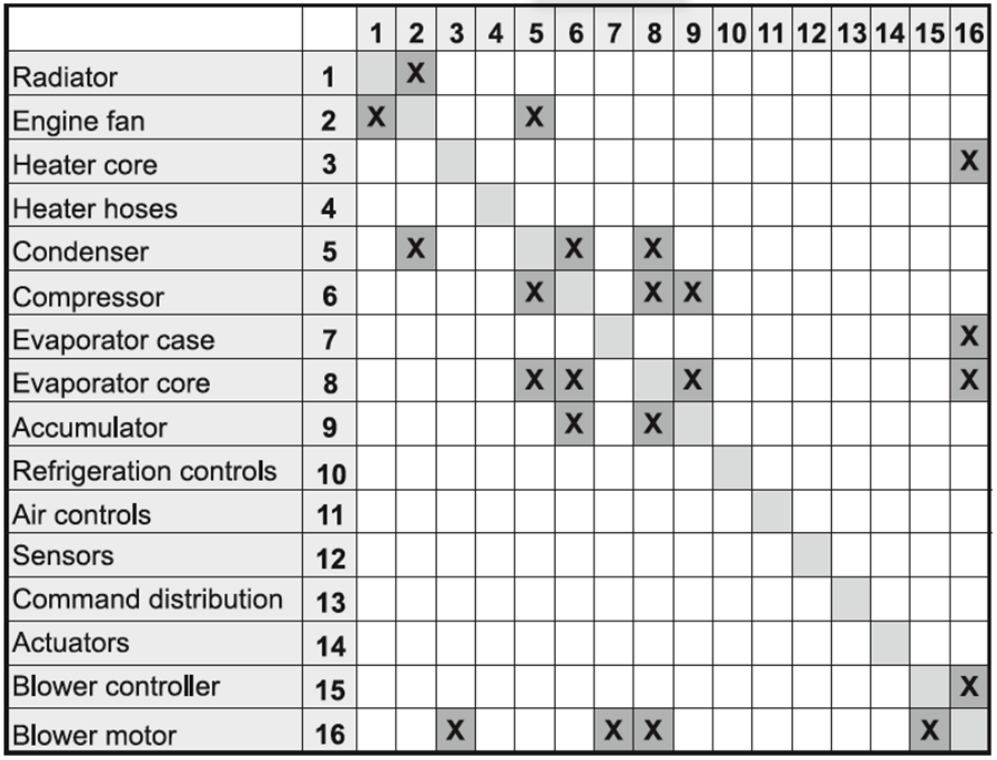
\includegraphics[width=0.6\linewidth]{Bilder/Teil3_KomponentenbasierteDSM.png}
                \caption{Komponentenbasierte DSM - Beispiel}
            \end{figure}
        \end{itemize}
    \item \textbf{Personenbasiert}
        \begin{itemize}
            \item Verbindung von Organisationseinheiten.
            \item Organisationsentwurf, Kommunikationsmanagement und Teamintegration.
            \begin{figure}[H]
                \centering
                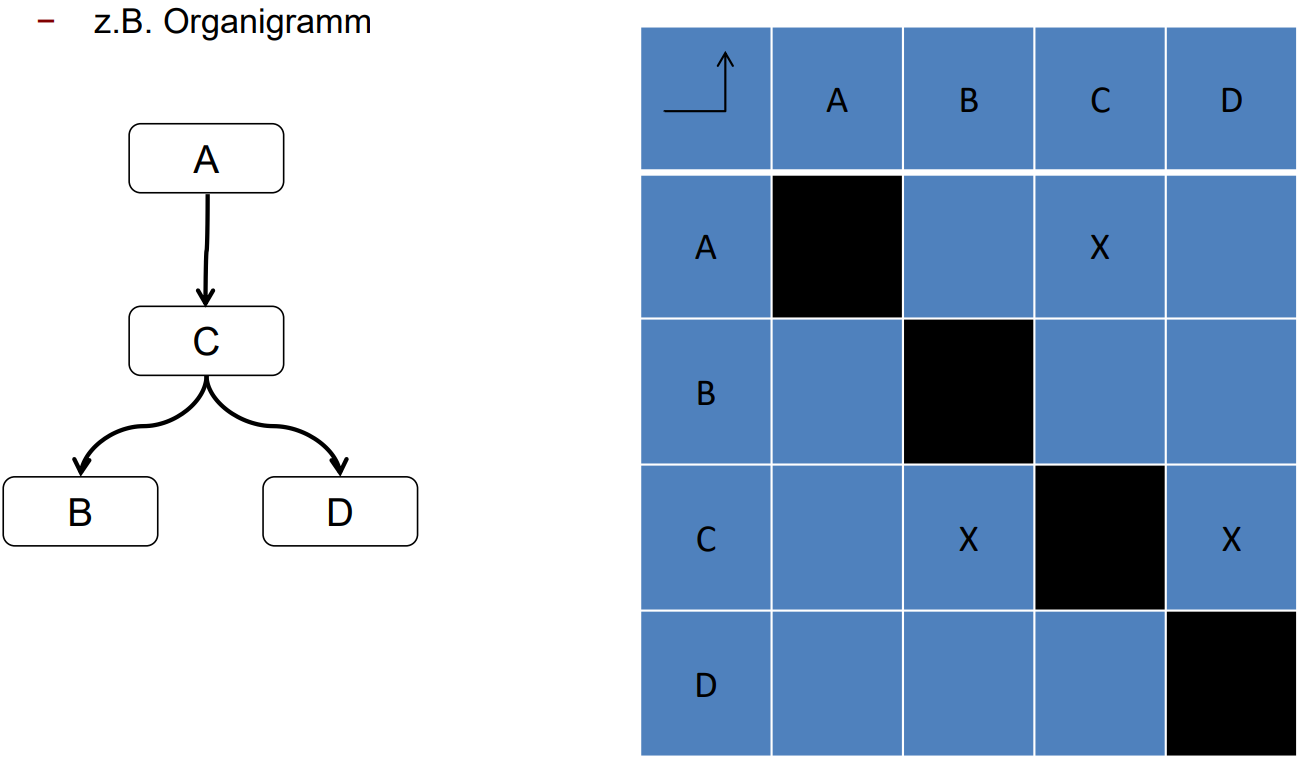
\includegraphics[width=0.6\linewidth]{Bilder/Teil3_PersonenbasierteDSM.png}
                \caption{Personenbasierte DSM - Beispiel}
            \end{figure}
        \end{itemize}
    \item \textbf{Aktivitätsbasiert}
        \begin{itemize}
            \item Verbindungen von Aktivitäten (Input / Output).
            \item Prozessverbesserung, Projektzeitplanung, Iterationsmanagement und Informationsflussmanagement.
            \begin{figure}[H]
                \centering
                \includegraphics[width=0.6\linewidth]{Bilder/Teil3_Aktivitätsbasierte DSM.png}
                \caption{Aktivitätenbasierte DSM - Beispiel}
            \end{figure}
        \end{itemize}
    \item \textbf{Parameterbasiert}
        \begin{itemize}
            \item Verbindungen von Design-Parametern.
            \item Aktivitätsabfolgen und Prozessentwurf.
            \begin{figure}[H]
                \centering
                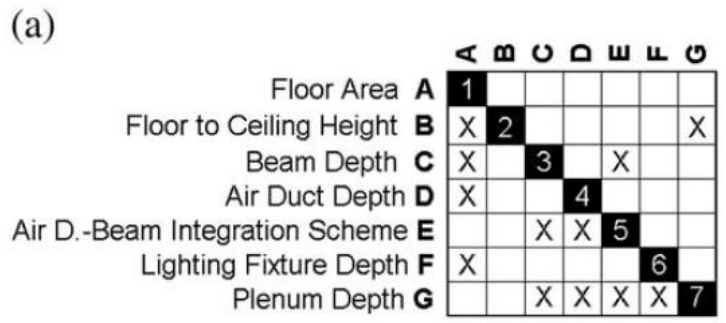
\includegraphics[width=0.6\linewidth]{Bilder/Teil3_ParameterbasierteDSM.png}
                \caption{Parameterbasierte DSM - Beispiel}
            \end{figure}
        \end{itemize}
\end{itemize}


% subsection
%-------------------------------------------------------------------------------------------
\subsection{Was bedeutet Sequenzierung von DSM?}

Sequenzierung ist die Umordnung der Zeilen und Spalten der DSM mit dem Ziel, dass es keine Schleifen gibt (Dreiecksmatrix).

\begin{itemize}
    \item Identifikation der Elemente ohne Information anderer Elemente ausgeführt werden könne.
        \\ Werden \textbf{nach links geschoben.}
    \item Identifikation die keine Information für andere Elemente liefert (Gegenteil von Punkt 1).
        \\ Werden \textbf{nach rechts geschoben.}
    \item Wenn Matrix nicht leer ist existiert mindestens eine Schleife. 
        \\ \textbf{Identifikations-Methoden:}
        \begin{itemize}
            \item Pfad Suchen.
            \item Adjazent Matrix.
            \item Erreichbarkeits Matrix Methode.
            \item Triangulations Algorithmus.
            \item Algorithms von Tarjan zur Bestimmung eines minimalen Spannungsbaumes.
        \end{itemize}
    \item \textbf{Beispiel einer Sequenzierung:}
        \begin{figure}[H]
            \centering
            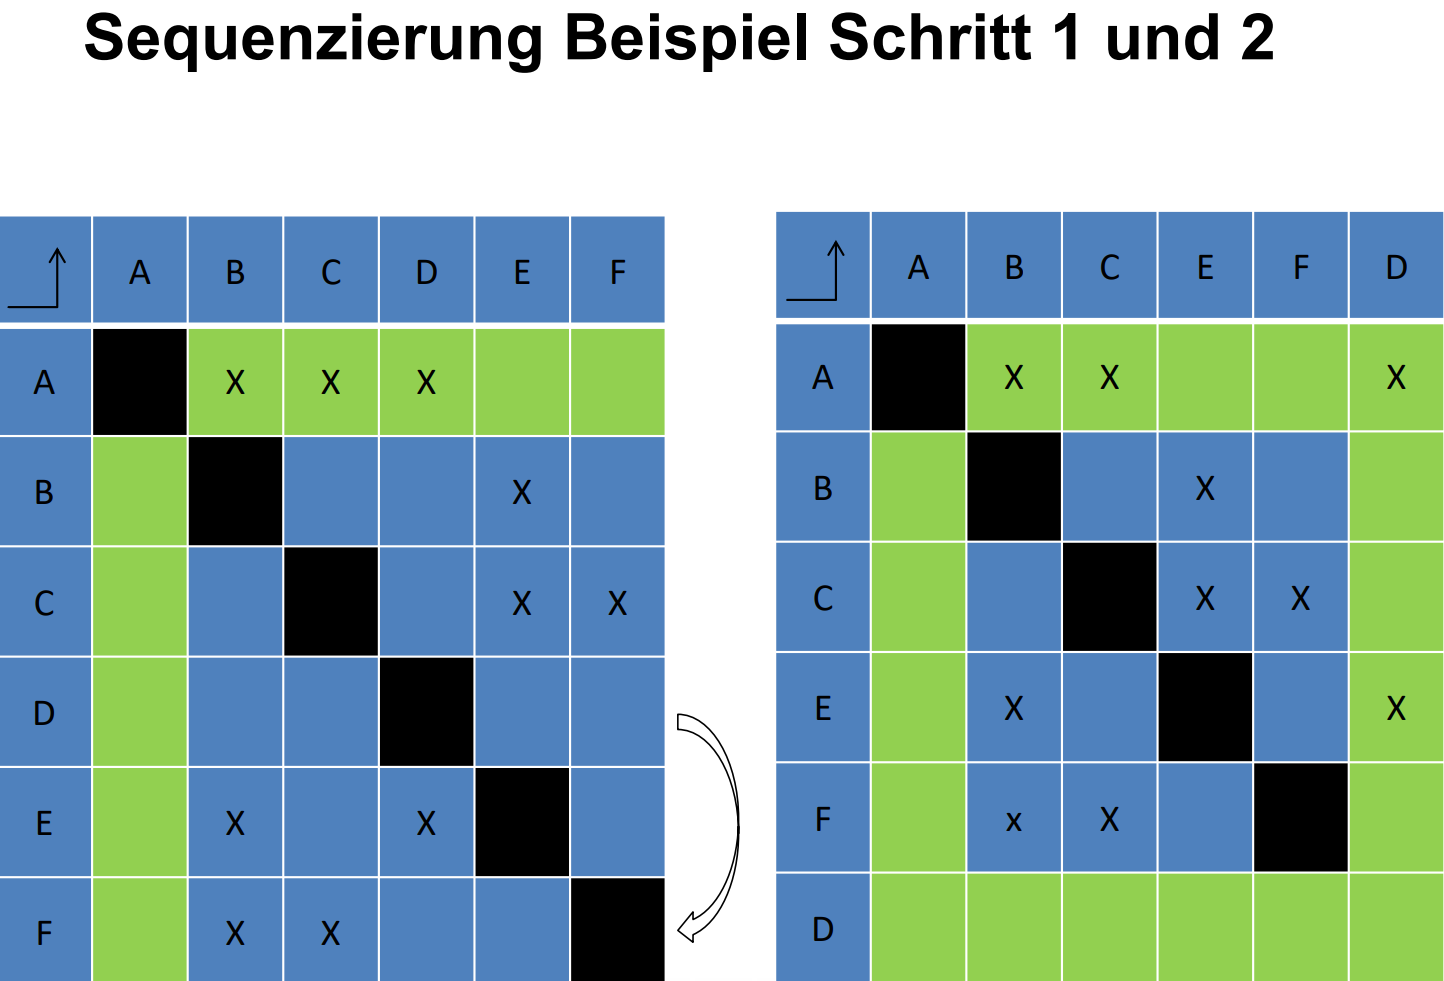
\includegraphics[width=0.8\linewidth]{Bilder/Teil3_SequenzierungBeispiel1.png}
            \caption{Sequenzierung Schritt 1 und 2 - Beispiel}
        \end{figure}
        \begin{figure}[H]
            \centering
            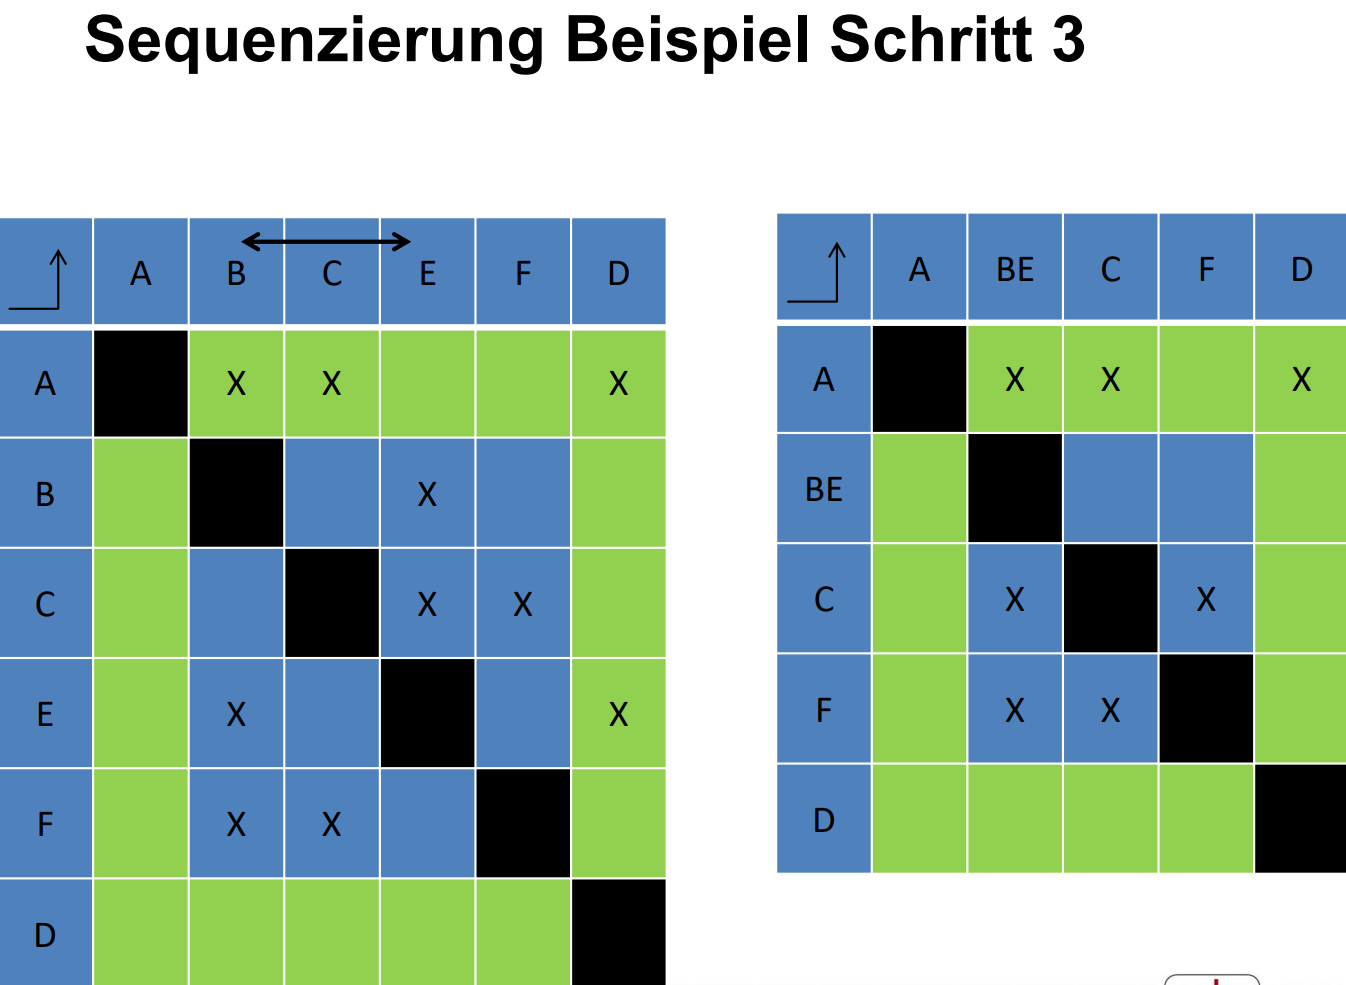
\includegraphics[width=0.8\linewidth]{Bilder/Teil3_SequenzierungBeispiel2.png}
            \caption{Sequenzierung Schritt 3 - Beispiel}
        \end{figure}
        \begin{figure}[H]
            \centering
            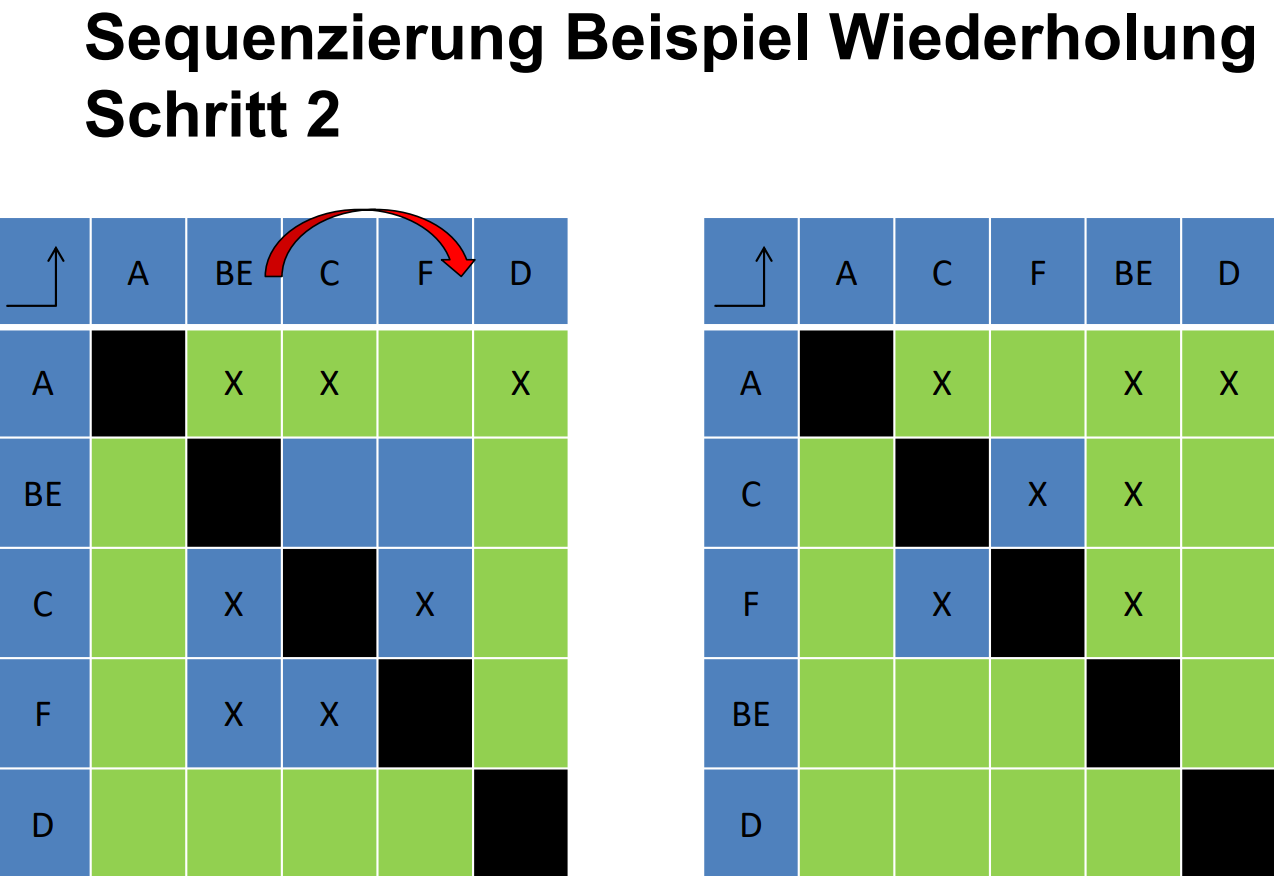
\includegraphics[width=0.8\linewidth]{Bilder/Teil3_SequenzierungBeispiel3.png}
            \caption{Sequenzierung Wiederholung Schritt 2 - Beispiel}
        \end{figure}
        \begin{figure}[H]
            \centering
            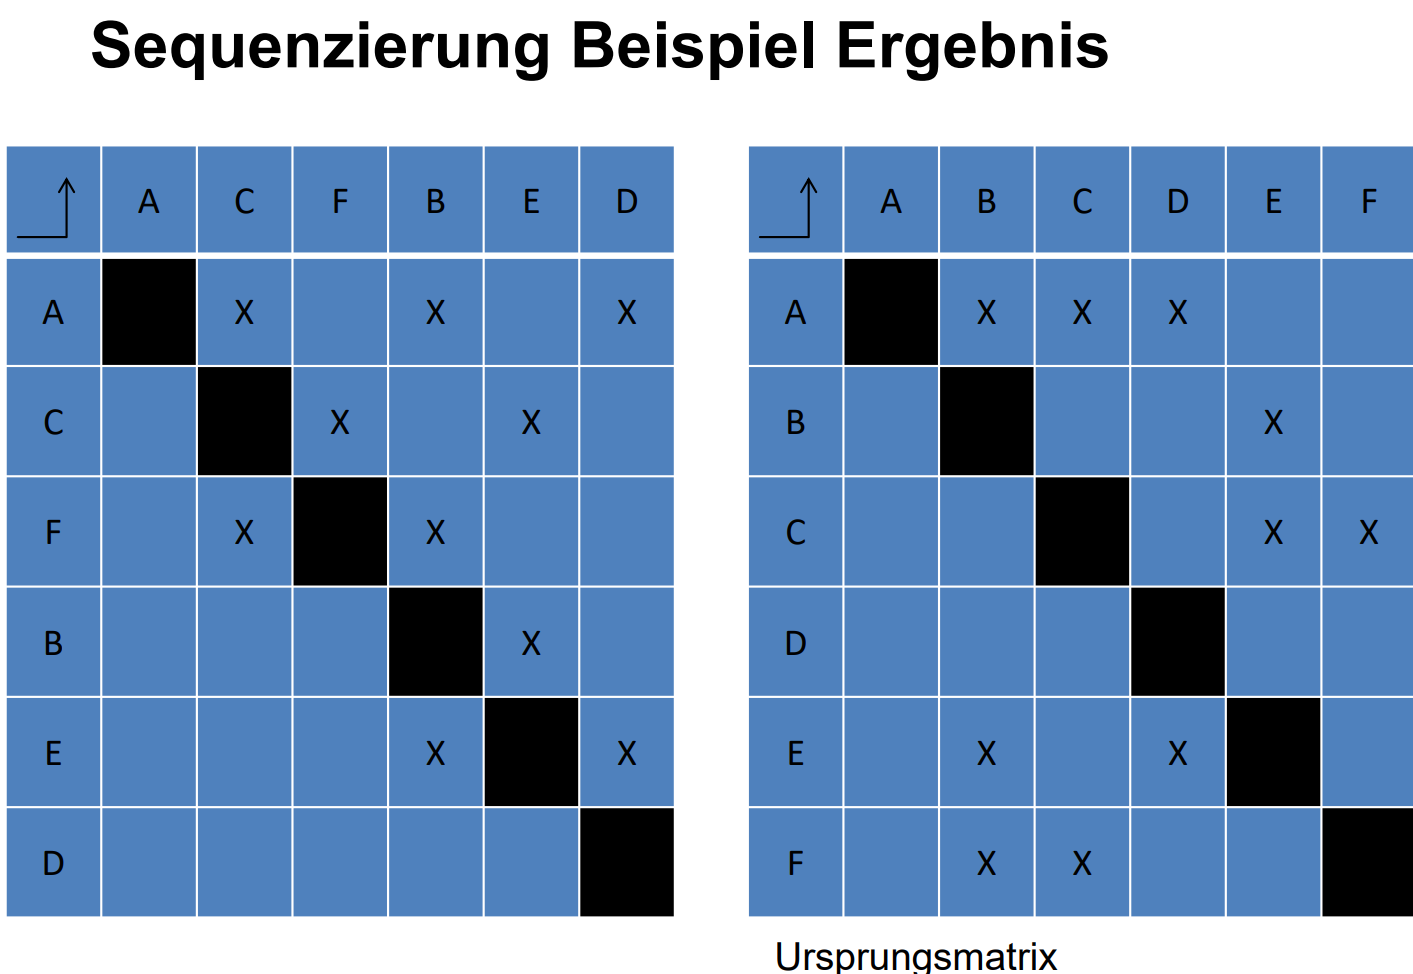
\includegraphics[width=0.8\linewidth]{Bilder/Teil3_SequenzierungBeispiel4.png}
            \caption{Sequenzierung Ergebnis - Beispiel}
        \end{figure}

        
\end{itemize}

% subsection
%-------------------------------------------------------------------------------------------
\subsection{Was bedeutet Clustering von DSM?}

Ziel ist es bei der Komponenten- bzw. Personenbasierten DSM \textbf{Cluster oder Module} zu identifizieren, in denen ein \textbf{Großteil der Interaktionen} stattfinden.

Clustering ermöglicht bessere Einblicke in die Teamorganisation und \textbf{Identifikation von Schlüsselparameter}.

\begin{figure}[H]
    \centering
    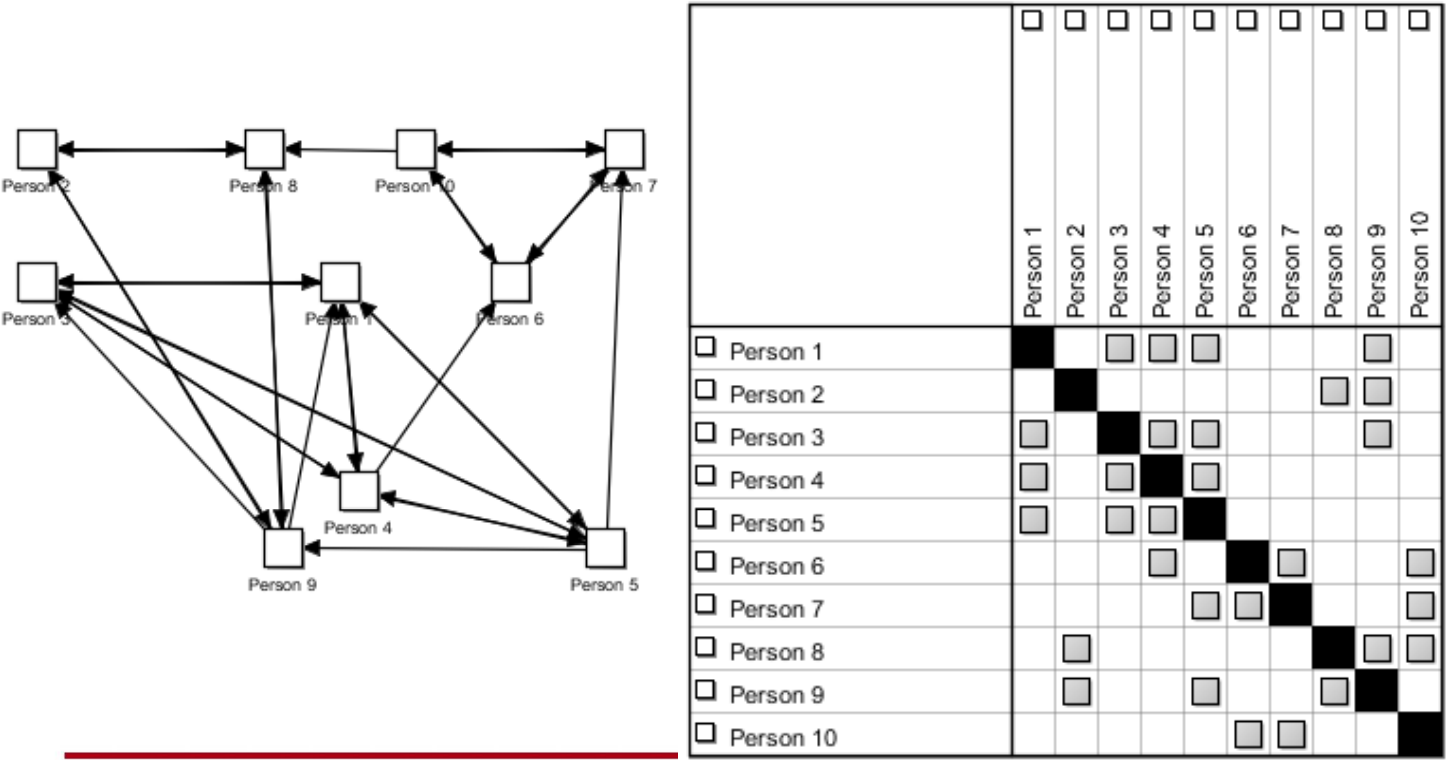
\includegraphics[width=0.8\linewidth]{Bilder/Teil3_ClusteringBeispiel.png}
    \caption{Clusterung - Beispiel}
\end{figure}

